\usetikzlibrary{arrows.meta,shapes.misc,shapes.geometric}
\begin{frame}{finding window size empirically (1)}
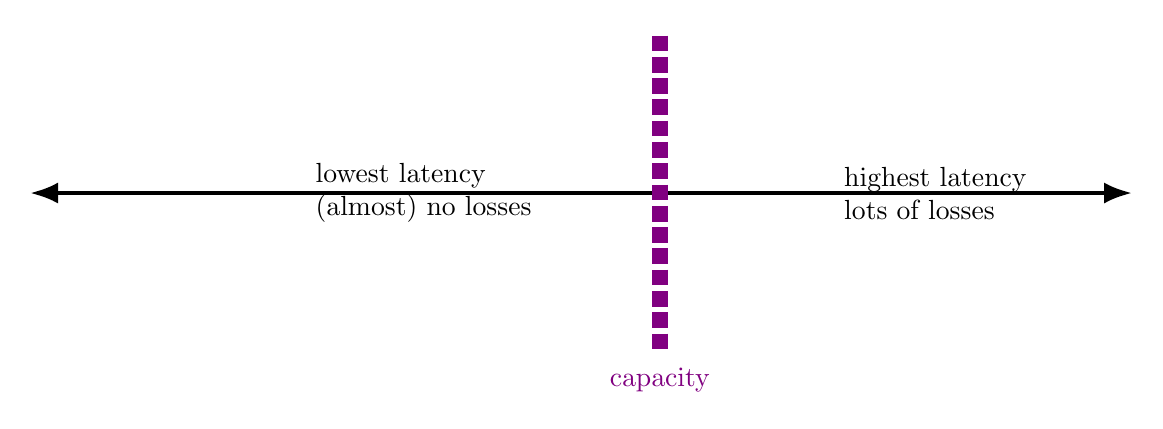
\begin{tikzpicture}
\draw[ultra thick,Latex-Latex] (-7, 0) -- (7, 0);
\draw[dotted,line width=2mm,violet] (1, 2) -- (1, -2) node[below] {capacity};
\node[align=left] at (-2, 0) {
    lowest latency \\
    (almost) no losses
};
\node[align=left] at (4.5, 0) {
    highest latency \\
    lots of losses 
};
\end{tikzpicture}
\end{frame}

\begin{frame}{key insight}
    \begin{itemize}
    \item latency/loss rate increases when window size too big
    \item latency/loss rate stable when window size not too big
    \vspace{.5cm}
    \item for now, we'll focus on loss rate
        \begin{itemize}
        \item but you can do something similar with latency
        \end{itemize}
    \end{itemize}
\end{frame}

\begin{frame}{try a bunch of things}
\begin{tikzpicture}
\tikzset{
    good/.style={draw,star,thick,fill=green!70!black},
    bad/.style={draw,cross out,red!70!black,line width=3mm},
}
\draw[ultra thick,Latex-Latex] (-7, 0) -- (7, 0);
\node at (0, -.5) {window size};
\node[good,label={east:= low loss rate}] (key good) at (-6, 2) {};
\node[bad,label={east:= high loss rate}] (key bad) at (-6, 1) {};
\begin{visibleenv}<2->
\node[good] at (-3, 0){};
\node[bad] (high bad) at (5, 0){};
\end{visibleenv}
\begin{visibleenv}<3->
\node[bad] at (1, 0){}; 
\end{visibleenv}
\begin{visibleenv}<4->
\node[good] at (-1, 0){}; 
\end{visibleenv}
\begin{visibleenv}<5->
\node[good] at (-0.5, 0){}; 
\node[good] at (-0.2, 0){}; 
\node[bad] at (0.3, 0){}; 
\node[bad] at (0.5, 0){}; 
\node[bad] at (0.9, 0){}; 
\end{visibleenv}
\begin{visibleenv}<6>
\draw[Latex-,very thick] (high bad) -- ++(-2, -5) node {
    what is the network like when we do this?
};
\end{visibleenv}
\end{tikzpicture}
\end{frame}
